\documentclass[11pt,letterpaper]{article}
\usepackage{jshbasic}
\usepackage{jshmaths}

\usepackage{multirow}
\usepackage{wrapfig}

\usepackage{framed}

\graphicspath{ {./figures/} }

\definecolor{lightgray}{gray}{0.83}

\newcommand{\panel}[1]{\colorbox{lightgray}{\textsf{#1}}}

\setcounter{tocdepth}{3}

\title{\textbf{\textsf{\huge{SeismoSoil Tutorial and Manual}}}}
\author{{\textsf{\Large{Domniki Asimaki}}}\thanks{Domniki Asimaki, Professor of Mechanical and Civil Engineering, California Institute of Technology.  \href{mailto:domniki@caltech.edu}{\textsf{domniki@caltech.edu}}, Website: \href{http://asimaki.caltech.edu}{\textsf{http://asimaki.caltech.edu}}}  \and {\textsf{\Large{Wei Li}}}\and {\textsf{\Large{Jian Shi}}}\thanks{Jian Shi, PhD student, Department of Mechanical and Civil Engineering, California Institute of Technology. Email: \href{mailto:jian.shi@caltech.edu}{\textsf{jian.shi@caltech.edu}}}}
\date{}


\begin{document}
  \maketitle
  \thispagestyle{empty}    % No page number on the first page
SeismoSoil is a site-specific response analysis software application, which performs 1-D linear elastic, equivalent linear, and nonlinear site response analyses.

\begin{framed}
	\begin{center}
		\textbf{By downloading or using this software, you acknowledge acceptance of the following DISCLAIMER OF WARRANTY:}
	\end{center}
	
	{\sffamily
			THIS SOFTWARE AND/OR RELATED MATERIALS ARE PROVIDED ``AS-IS'' WITHOUT WARRANTY OF ANY KIND. WE MAKE NO WARRANTIES, EXPRESS OR IMPLIED, THAT THEY ARE FREE OF ERROR, OR ARE CONSISTENT WITH ANY PARTICULAR BUILDING CODES AND/OR STANDARDS, OR ARE SUITABLE FOR A PARTICULAR USE OR PURPOSE OR FOR ANY PURPOSE WHATSOEVER, HOWEVER USED.
			
			IN NO EVENT SHALL THE CALIFORNIA INSTITUTE OF TECHNOLOGY OR THE AUTHORS OF THIS SOFTWARE BE LIABLE FOR ANY DIRECT, INDIRECT, INCIDENTAL, SPECIAL, EXEMPLARY, OR CONSEQUENTIAL DAMAGES (INCLUDING, BUT NOT LIMITED TO, PROCUREMENT OF SUBSTITUTE GOODS OR SERVICES; LOSS OF USE, DATA, OR PROFITS; DAMAGE TO COMPUTING EQUIPMENT, COMPUTER SYSTEMS, SOFTWARE, OR STORED DIGITAL DATA; OR BUSINESS INTERRUPTION) HOWEVER CAUSED AND ON ANY THEORY OF LIABILITY, WHETHER IN CONTRACT, STRICT LIABILITY, OR TORT (INCLUDING NEGLIGENCE OR OTHERWISE) ARISING IN ANY WAY OUT OF THE USE OF THIS SOFTWARE, EVEN IF ADVISED OF THE POSSIBILITY OF SUCH DAMAGE.
			
			USER BEARS ALL RISK RELATING TO QUALITY AND PERFORMANCE OF THIS SOFTWARE AND/OR RELATED MATERIALS.
			
	}
	
	\vspace{0.5cm}
\end{framed}

\begin{center}
	\textcopyright\quad 2015 California Institute of Technology
\end{center}
%System requirements\\
%Operating system: 64-bit Windows (Mac and Linux versions are on their way)\\
%Available disk space: 3 GB (please also note that the output files are fairly large)\\
%Note: MATLAB Compiler Runtime is required to run SeismoSoil (see Section 2)\\

\newpage
\tableofcontents

\newpage
\section{Introduction}

SeismoSoil is a one-dimensional (1D) site response analysis simulation and visualization application.

\subsection{Main features}
%The main features of SeismoSoil includes the following:
\begin{itemize}
    \item \textbf{\textsf{Linear analysis}}
        \begin{itemize}
            \item Frequency domain analysis, which performs the most basic and simplest type of analysis, following the Haskell-Thompson formulation
            \item Time domain analysis, useful when the ``wrap-around'' phenomenon of Fourier transform is pronounced and needs to be addressed
        \end{itemize}
    \item \textbf{\textsf{Equivalent linear analysis (frequency domain)}}
        \begin{itemize}
            \item Original Seed and Idriss (1970) equivalent linear method
            \item Frequency dependent moduli and damping method (Assimaki \& Kausel, 2002)
        \end{itemize}
    \item \textbf{\textsf{Nonlinear analysis (time domain)}}
        \begin{itemize}
            \item \emph{H2}: Masing unloading/reloading rule + modified hyperbolic stress-strain model (MKZ), or
            \item \emph{H4}: Muravskii (2005) unloading/reloading rule (non-Masing) + MKZ
            \item (Built-in tools for doing \emph{H2} and \emph{H4} curve fitting)
            \item \emph{EPP}: Masing unloading/reloading rule + elasto-perfectly plastic stress-strain model
        \end{itemize}
    \item \textbf{\textsf{Auto-generation of modulus reduction and damping curves}}
        \begin{itemize}
            \item Generates depth-dependent $G/G_{\text{max}}$ and damping curves directly from the soil property profile
            \item Based on the formulas proposed by Darendeli (2001)
        \end{itemize}
    \item \textbf{\textsf{Various tools that aid the simulation of site response}}
        \begin{itemize}
            \item Baseline correction, digital signal filtering
            \item Motion deconvolution, response spectra calculations, etc.
        \end{itemize}
    \item \textbf{\textsf{Fast and easy-to-use graphical user interface (GUI)}}
        \begin{itemize}
            \item The GUI is intuitive and self-explanatory
            \item SeismoSoil utilizes parallel computing technique, using all the cores of the CPU, enabling fast processing speed even for nonlinear analyses
            \item All input and output data files are in plain text format, allowing easy pre-processing and post-processing in Excel/MATLAB/Python/etc.
            \item Figures generated can be directly saved to the hard drive
        \end{itemize}
\end{itemize}

%It offers the following options: frequency domain linear viscoelastic, equivalent linear, and finite difference time domain linear and nonlinear analyses. For the latter, it has built-in frequency independent damping for low strains, and automatic model parameter fitting to the nonlinear dynamic soil properties ($G/G_{\max}$ and damping).

%In addition, SeismoSoil offers motion deconvolution from rock outcrop to borehole (through viscoelastic layered bedrock), and allows input motion definition in three ways: (i) borehole motion (also known as motion ``within'' or total motion at depth); (ii) incident motion at depth (free of downgoing waves, useful for integration of site response in seismological model predictions); and (iii) rock outcrop (RO) motion; if the rock outcrop site has its separate site response (that is to say, for stations on the surface of viscoelastic homogeneous or layered media), motion should be deconvolved from RO to incident before performing site response.

%The toolbox also includes functions such as Fourier and Elastic Response Spectra, Arias Intensity, linear transfer functions, baseline correction and signal filtering (low pass, high pass and band pass filters).

%Output results include ASCII files of acceleration, velocity, displacement, stress and strain time histories at each layer, and maximum values with depth; visualization output includes time histories, Fourier and response spectra of ground motion on the surface, and maximum acceleration, velocity, displacement, stress and strain with depth.

\newpage
\subsection{Functionality structure}

\begin{figure}[H]
\centering
  % Requires \usepackage{graphicx}
  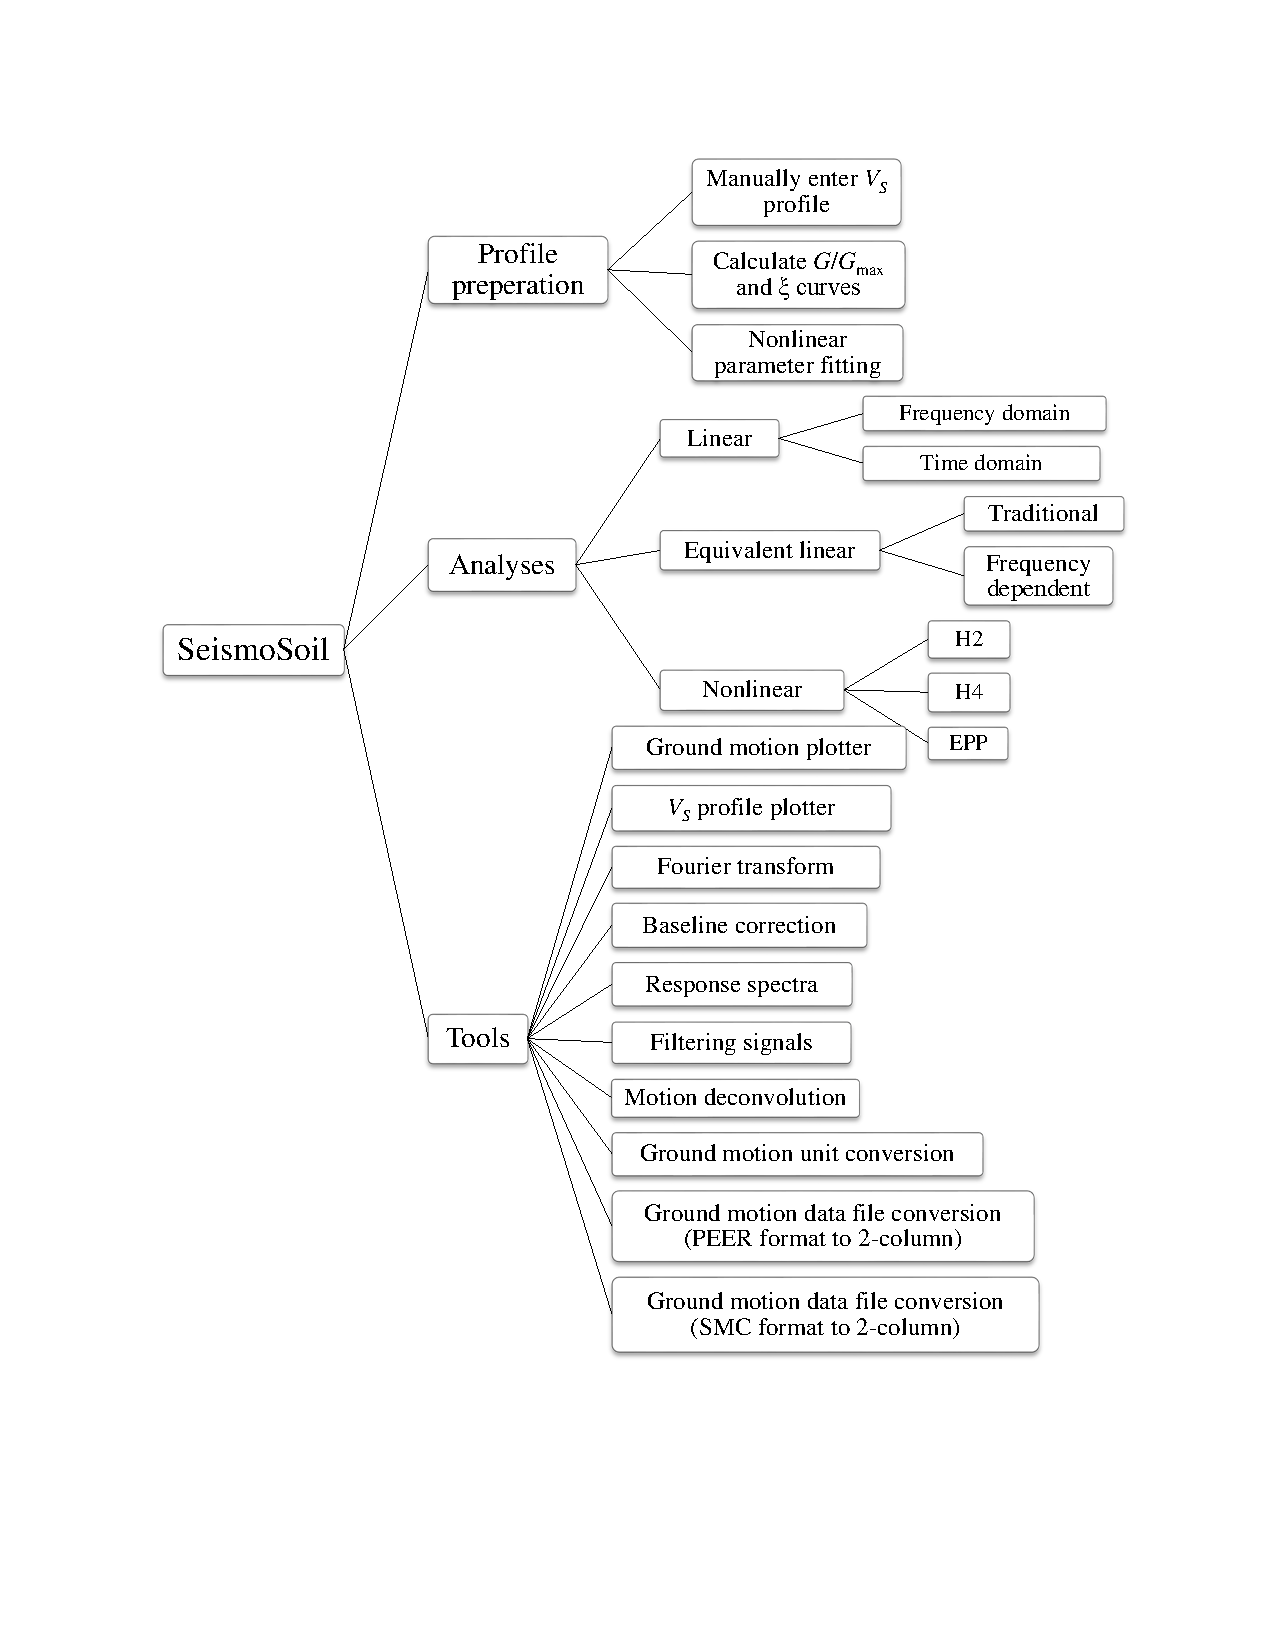
\includegraphics[width=.99\textwidth]{functionality_structure.pdf}\\
  %\caption{}\label{}
\end{figure}

%\newpage
\section{User Tutorial}
\subsection{Launch SeismoSoil}

\subsubsection{Windows users}

\begin{enumerate}
	\item Install MATLAB Compiler Runtime (MCR), which can be downloaded from MathWorks website for free\footnote{\href{http://www.mathworks.com/products/compiler/mcr}{\textsf{http://www.mathworks.com/products/compiler/mcr}} (please choose ``R2014a (8.3), 64-bit'')}. If your MATLAB version is R2014 64-bit, then you can skip this step.
	
	\item Open {\textsf{{SeismoSoil\_[version number].exe}}}. (Please keep the four auxiliary files, {\textsf{TDLinear.exe}}, {\textsf{FDEQ.exe}}, {\textsf{NLH2.exe}} and {\textsf{NLH4.exe}}, in the same directory as {\textsf{{SeismoSoil.exe}}})
\end{enumerate}

\subsubsection{Mac OS X users}

\begin{enumerate}
	\item Install MATLAB Compiler Runtime (MCR), which can be downloaded from MathWorks website for free (see footnote). If your MATLAB version is R2014 64-bit, then you can skip this step.
	
	\item Place the APP file (the file with the MATLAB icon) in the Applications folder.
	\item From Terminal, execute the following (without the quotation marks):\\
	 ``\texttt{/Applications/SeismoSoil.app/Contents/MacOS/applauncher}''. \\(Please start SeismoSoil only from the Terminal. If you open it by double-clicking the icon, some unexpected errors will occur during runtime.)
\end{enumerate}

The system requirement of SeismoSoil is: Windows (64-bit) or Mac OS X (64-bit Mavericks or Yosemite), with enough disk space (recommended 4~GB). There is no requirement for minimum CPU and memory, but SeismoSoil runs much faster on more advanced machines (especially with more cores).

The screenshot of the \panel{main} panel of SeismoSoil, shown on the next page, will appear after startup.

\subsection{Input files preparation}

Input file examples are provided in the folder ``Sample Input Files''. Users can start trying SeismoSoil right away using these files, or can follow the following paragraphs in this section to learn to prepare new input files.

All input files are in plain text format (for example, \textsf{.txt} files). Acceptable delimiters include spaces, commas, and horizontal tabs. The output files generated by SeismoSoil will have horizontal tabs as delimiters.

\begin{figure}[H]
\centering
  \includegraphics[width=.8\textwidth]{main.png}\\
\end{figure}

\newpage
\subsubsection{Ground motion}\label{sec:motion_file}

Ground motion data files that can be read by SeismoSoil should have two (and only two) columns---the left column is the time vector in units of seconds, and the right column is the acceleration, in units of $\ein{m/s^2}$, gal ($=1\ein{cm/s^2}$), or $g$ ($=9.81\ein{m/s^2}$). Users can choose their corresponding unit in simulation graphical panels. There is a \panel{NGA to 2-column converter} panel under \panel{main}$\rightarrow$\panel{tools}, which converts the~\textsf{.AT2} format used by PEER/NGA database into the 2-column format.

\panel{Main}$\rightarrow$\panel{tools}$\rightarrow$\panel{ground motion plotter} provides plots of acceleration time history, as well as velocity and displacement time histories, which are integrated from the acceleration. Arias intensity and RMS acceleration can also be calculated. An example output of the \panel{ground motion plotter} is shown below.

\begin{figure}[H]
\centering
  \includegraphics[width=.56\textwidth]{ground_motion_plot.png}\\
\end{figure}

Under \panel{main}$\rightarrow$\panel{tools}, users can also find \panel{signal filter} and \panel{baseline correction}, which filter or baseline-correct the ground motion accelerations; in addition, they can plot the Fourier spectra with \panel{Fourier transform} and elastic response spectra (with any damping ratio value) with \panel{elastic response spectra}. An example of the baseline correction output is shown below. The algorithm of the baseline correction is listed in Section \ref{sec:baseline-correction}.

\begin{figure}[H]
\centering
  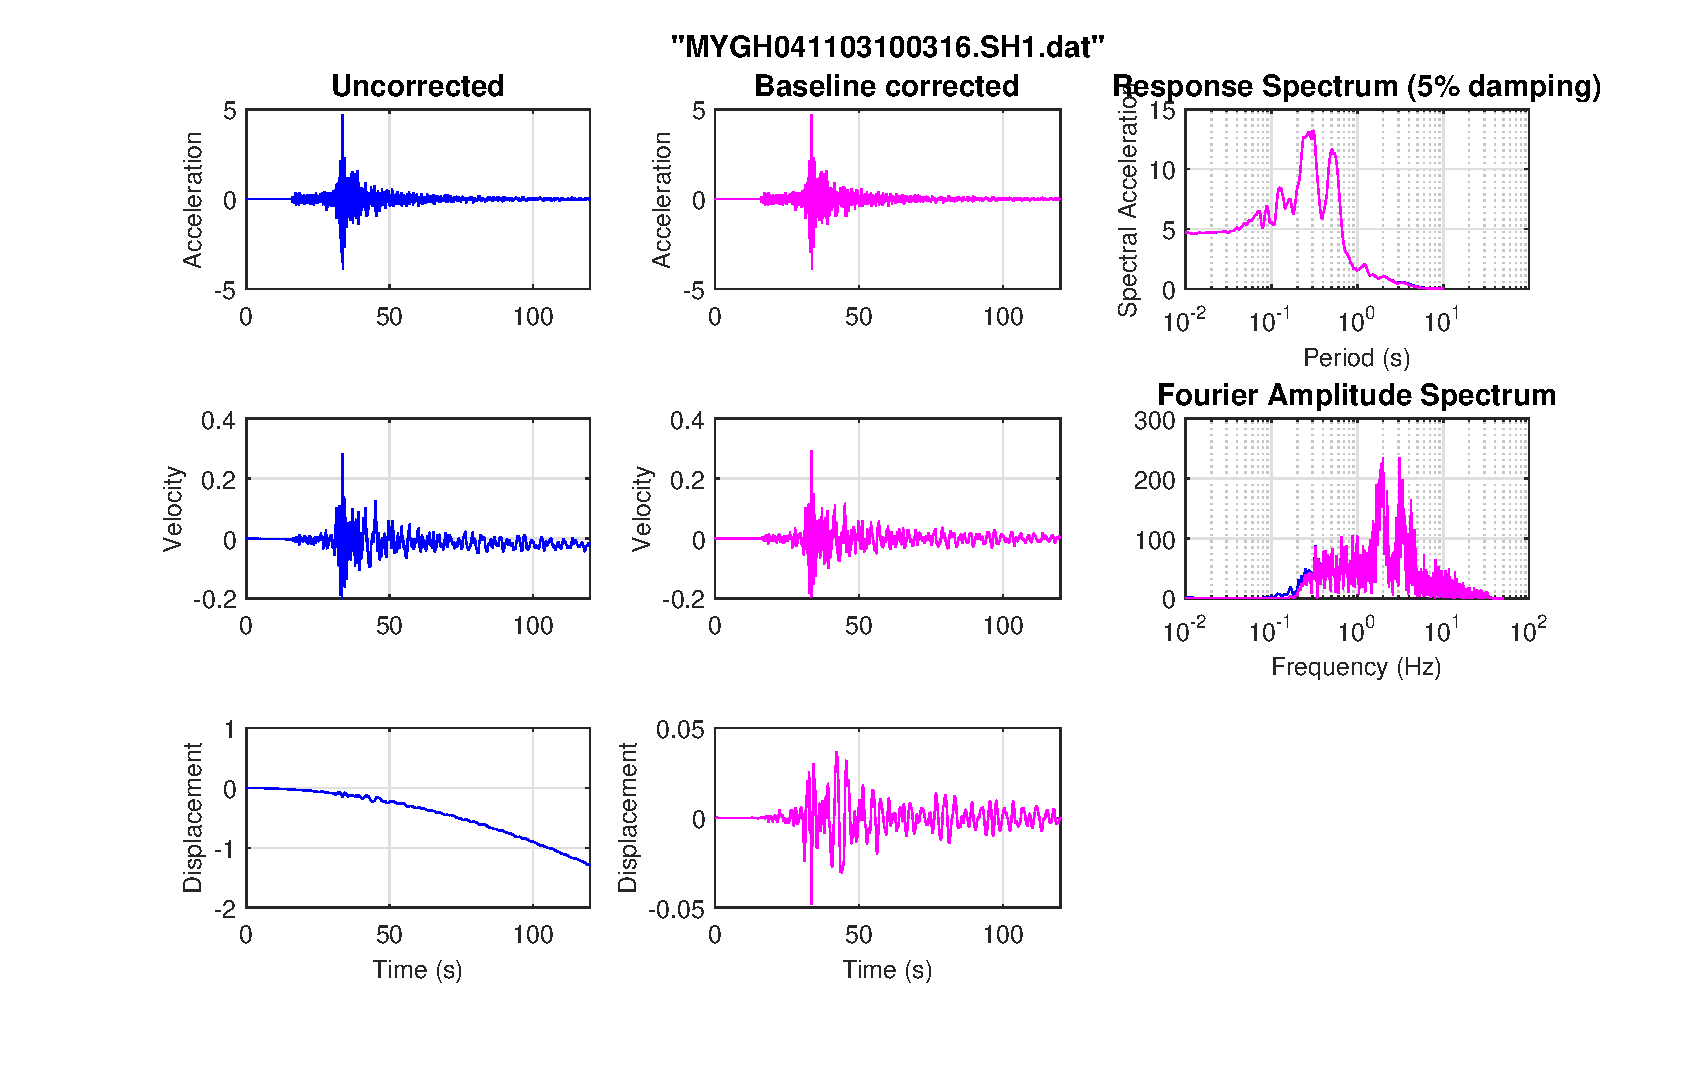
\includegraphics[width=.99\textwidth]{baseline_correction_result_new.eps}\\
  \label{fig:baseline_result}
\end{figure}

\subsubsection{Soil profile}\label{sec:soil_profile}

The input file containing the soil property profile should be in the following five-column format:

\begin{figure}[H]
\centering
  \includegraphics[width=.62\textwidth]{profile_file.png}\\
\end{figure}

From left to right, the columns mean: soil layer thickness (m), shear wave velocity $V_s$ (m/s), low-strain damping ratio, $\xi$, soil mass density, $\rho$, and ``material number'', respectively. The units of $\xi$ can be either \% or unity (i.e., 1), and the unit of $\rho$ can be either $\ein{g/cm^3}$ or $\ein{kg/m^3}$. The users can specify the units of $\xi$ and $\rho$ on the simulation panels, before the analysis starts. The last thickness value \emph{should always be 0}, which indicates the last layer (i.e., the halfspace) has infinite depth.

The fifth column, the ``material number'', should be a series of positive integers, not necessary in a continuous and ascending order, with the exception of the last value, which \emph{should always be 0}. The material number refers to the nonlinear dynamic soil parameters, namely the $G/G_{\max}$ and damping curves. For example, the layers with ``material number''=5 correspond to the 5th set of $G/G_{\max}$ and damping curves in the ``curve file'', which will be explained in Section \ref{sec:curve}.

The soil profile can be manually entered through \panel{main}$\rightarrow$\panel{profile preparation}$\rightarrow$\panel{manually enter Vs profile}. A screenshot of this panel is shown below.  Alternatively, users can prepare the input files in external applications like Excel or Notepad, and save them as plain text files.

\begin{figure}[H]
\centering
  \includegraphics[width=\textwidth]{profile_prepare.png}\\
\end{figure}

\subsubsection{Nonlinear dynamic soil properties: $G/G_{\max}$ and damping ratio curves}\label{sec:curve}

The two input files mentioned in Sections \ref{sec:motion_file} and \ref{sec:soil_profile} are the only files required for linear site response analysis. For the equivalent linear and nonlinear analyses options, dynamic soil properties $G/G_{\max}$ and $\xi$ of soils are required. In SeismoSoil, these properties are specified in a single text file (the ``curve file'').

Below is the format of a ``curve file''. The headers are just for demonstration and should not be included in the actual ``curve file''.

\begin{figure}[H]
\centering
  \includegraphics[width=.81\textwidth]{curve_file_format.png}\\
\end{figure}

Each group of four columns corresponds to the dynamic nonlinear soil properties of one material: $G/G_{\max}$ and $\xi$ vs shear strain. The material number, $k$, on the fifth column of the input soil profile file corresponds to the $k$-th set of 4 columns in the ``curve file''.

In \panel{main}$\rightarrow$\panel{profile preparation}$\rightarrow$\panel{modulus and damping (Darendeli, 2001)}, the $G/G_{\max}$ curves and $\xi$ curves can be automatically calculated using M.~B.~Darendeli's (2001)\footnote{Darendeli, M.~B.~(2001). ``Development of a new family of normalized modulus reduction and material damping curves.'' Pages 220--272, \emph{PhD thesis}, The University of Texas at Austin.} formulas The assumptions are:
\begin{itemize}
\item Total stress analysis (deep groundwater table)
%\item PI (plasticity index) = 20\%
\item OCR: 1.0 (normally consolidated)\footnote{The users are welcome to contact us, if they would like to calculate curves using different OCR, $N$, or $f$ values.}
\item $N$ (number of cycles): 10
\item $f$ = 1 Hz
\end{itemize}

Thus, the only variable that governs the nonlinear dynamic soil properties is the overburden pressure, which is internally calculated using mass density and depth information.

The ground motion, soil profile and nonlinear dynamic soil properties are the necessary input files for equivalent linear analyses. For nonlinear analyses, the users should also specify the constitutive model parameters, as will be discussed in \ref{sec:para}.

\subsubsection{Nonlinear constitutive soil model parameters}\label{sec:para}

%The constitutive soil model in SeismoSoil is the generalized modified hyperbolic model (MKZ), originally proposed by Matasovic and Vucetic (1993)\footnote{Matasovic, N., and Vucetic, M.~(1993) ``Cyclic Characterization of Liquefiable Sands.'' \emph{ASCE Journal of Geotechnical and Geoenvironmental Engineering}, 119(11), 1805--1822.} and later modified by Hayashi et al.~(1992)\footnote{Hayashi, H., M.~Honda, and T.~Yamada.~(1992) ``Modeling of nonlinear stress strain relations of sands for dynamic response analysis.'' \emph{In Proceeding: 10th World Conference on Earthquake Engineering}, Volume 11, Pages 6819--6825, Madrid, Spain, Balkema, Rotterdam.}. In addition, it includes two hysteretic rules, hereby denoted \emph{H2} and \emph{H4}.
%
%\begin{figure}[H]
%\centering
%  % Requires \usepackage{graphicx}
%  \includegraphics[width=.45\textwidth]{H2_fit.png}\\
%  %\caption{}\label{}
%\end{figure}
%
%\emph{H2} is replicates the traditional Masing rules; this means that the backbone curve is derived as the integral of the modulus degradation curve (to which MKZs parameters are calibrated) and successively, the damping of the model is derived from translated and scaled replicas of the monotonic curve. This ensures perfect fitting of the modulus degradation curve, and overestimates the damping at large strains (see the figure above).
%
%\emph{H4} on the other hand is based on an extension of the Muravskii (2005)\footnote{Muravskii, G.~(2005) ``On description of hysteretic behavior of materials.'' \emph{International Journal of Solids and Structures}, Vol.~42, Nos.~9--10, 2625--2644.} hysteresis model, which updates the parameters of unloading and reloading at each stress reversal to match the damping vs strain curve, independently of the monotonic parameters. However, this approach has been shown to cause numerical instabilities and spurious high frequency resonances at large strains. In our version, the unload-reload parameters are calibrated once for the same functional form as the monotonic loading, prior to the analysis, and are thereafter kept constant during the simulations. This process is done in stages; first we fit the modulus reduction, and then the damping parameters (see the figure below). Successively, when the model is loaded, the constitutive law uses the loading parameters, and during unloading it uses the unloading parameters that are calibrated from the damping curve (see the figure below). While this approach compromises the fitting between model and experimental results, it has been shown to perform much better than the Muravskii alternative in large strains.
%
%\begin{figure}[H]
%\centering
%  % Requires \usepackage{graphicx}
%  \includegraphics[width=.80\textwidth]{H4_fit.png}\\
%  %\caption{}\label{}
%\end{figure}
%
%In general, we recommend the use of \emph{H2} for intermediate strain problems ($10^{-2}$) and the use of \emph{H4} for large strain ($>10^{-2}$) problems.
%\texttt{H2\_n.txt} is the input file for \emph{H2}, and \texttt{H4\_G.txt} and \texttt{H4\_x.txt} are the input files for \emph{H4} (two sets of parameters).

Apart from the ground motion, soil profile, dynamic curves, the nonlinear analysis in SeismoSoil requires additional information---the constitutive soil parameters. The \emph{H2} nonlinear method requires one file, \textsf{H2\_n.txt}, and the \emph{H4} nonlinear method requires two files, \textsf{H4\_G.txt} and \textsf{H4\_x.txt}.  These files have the same format, which looks like below (actual input files should not have the table headers):

\begin{figure}[H]
\centering
  \includegraphics[width=.52\textwidth]{H2_n_format.png}\\
\end{figure}

Each column of the file corresponds to a set of 4 columns in the ``curve file'', and in the same order as the ``curve file''. $\gamma_{\text{ref}}$ is the reference strain, and $s$ and $\beta$ are the two parameters in the MKZ model. These three parameters are obtained by curve-fitting the two predefined hysteretic models (\emph{H2} and \emph{H4}).

Curve fitting can be done using the \panel{main}$\rightarrow$\panel{profile preparation}$\rightarrow$\panel{nonlinear curve fitting} panel (shown in the figure below), which takes a ``curve file'' as the input, and generates a \textsf{H2\_n.txt} file (using \emph{H2} curve fitting) or \textsf{H4\_G.txt} and \textsf{H4\_x.txt} files (using \emph{H4} curve fitting).

The details of the MKZ model, the two unloading/reloading rules and these curve-fitting parameters will be explained in Section~\ref{sec:manual}, the technical manual.


\begin{figure}[H]
\centering
  \includegraphics[width=.7\textwidth]{nonlinear_curve_fitting.png}\\
\end{figure}

%Select the ``curve file'', and click either \colorbox{lightgray}{H2 fitting \& save} or \colorbox{lightgray}{H4 fitting \& save}. Because the curve fitting uses an optimization scheme (genetic algorithm with local hill climbing), it is generally slow.

\newpage
\subsection{Run the simulation}

The input files necessary for different kinds of simulations are summarized below.

\begin{small}
\begin{table}[H]
    \centering
%  \caption{}\label{}
    \begin{tabular}{|c|c|c|c|c|c|c|c|}
         \hline
         & & profile & motion & curve & H2\_n & H4\_G & H4\_x \\
         \hline
        \multirow{2}{*}{Linear} & frequency domain & \checkmark & \checkmark &   &   &  & \\
        \cline{2-8}
         & time domain & \checkmark & \checkmark &   &   & &\\
         \hline
         \multirow{2}{*}{Equivalent linear} & Seed \& Idriss (1970) & \checkmark & \checkmark & \checkmark  &   &   &\\
        \cline{2-8}
         & frequency dependent & \checkmark & \checkmark & \checkmark &   &  &\\
         \hline
         \multirow{2}{*}{Nonlinear} & H2 & \checkmark & \checkmark & \checkmark  & \checkmark  &   &\\
        \cline{2-8}
         & H4 & \checkmark & \checkmark & \checkmark &   & \checkmark & \checkmark \\
         \hline
    \end{tabular}
\end{table}
\end{small}


%For linear analyses, the user needs only the soil profile and the input motion. For equivalent linear analysis, the user needs the soil profile, the soil curves file, and the input motion. For nonlinear analysis with Masing rules (\emph{H2}), the users need the soil profile, curves file, \texttt{H2\_n} file, and the motion; and with modified hysteretic rule (\emph{H4}), the users need the soil profile, curves file, \texttt{H4\_G} file, \texttt{H4\_x} file, and the input motion.

%The screenshot below is the panel for a nonlinear \emph{H4} analysis. Follow each steps indicated on the panel, import all necessary input files, and click \colorbox{lightgray}{Start}. You can adjust the name of the soil profile, some of the input units, choose a baseline correction option, and select the output directory. The user is advised to carefully choose the type of bedrock (elastic or rigid) and the location that the input motions are prescribed or incident or recorded. Please refer to Section 5 for more details.

The user interface for linear analysis is shown below. The users can follow ``step 1'' to ``step 3'' on the panel and import the corresponding data. And then the users can click \textsf{Start} to start the calculation. Time-domain and frequency-domain linear methods both have the same user interface.

Please note that in Step 1.2 and Step 3.2, bedrock type and motion type should be chosen. Careful consideration is strongly recommended here, since different combinations of these two can lead to rather different results.  Please refer to the notes in Section~\ref{sec:bedrock-type-and-motion-location} on page \pageref{sec:bedrock-type-and-motion-location} for a detailed explanation of how to make the choice.

\begin{figure}[H]
\centering
  % Requires \usepackage{graphicx}
  \includegraphics[width=0.99\textwidth]{linear_panel.png}\\
  %\caption{}\label{}
\end{figure}


\newpage
The user interface for equivalent linear (traditional and frequency dependent) methods is shown below. Similarly to the linear analysis, the users can follow the procedures indicated on the panel and import the corresponding data.

\begin{figure}[H]
\centering
  % Requires \usepackage{graphicx}
  \includegraphics[width=0.99\textwidth]{equivalent_linear_panel.png}\\
  %\caption{}\label{}
\end{figure}

On the bottom-right corner of the panel, there are two check-box options. The second check box is self-explanatory, and the first check box controls whether figures of the simulation results will pop out. Note that the same figures will always be saved to the hard drive as PNG format.

\newpage
The user interface for \emph{H4} nonlinear analysis is shown below. The users should have no problem following the procedures indicated on the panel and import the corresponding data. The interface for \emph{H2} nonlinear analysis differs slightly with \emph{H4}, only in ``step 3'', where \emph{H2} only requires one input file, namely, \textsf{H2\_n.txt}.

\begin{figure}[H]
\centering
  % Requires \usepackage{graphicx}
  \includegraphics[width=0.99\textwidth]{H4_panel.png}\\
  %\caption{}\label{}
\end{figure}

\subsection{Notes on parallel computing}

Note that, on the bottom-right corner of the panel, there are two additional check boxes. ``Use multiple CPU cores'' controls whether or not SeismoSoil utilizes multiple cores of your CPU. If this box is checked, multiple ground motions will be processed in your CPU simultaneously, making the simulation approximately $n$ times faster, where $n$ is the total number of cores (not threads) of your CPU.

\subsection{Notes on Fortran kernel}

The box ``Use Fortran for calculation (faster)'' is checked by default. When checked, SeismoSoil calls the Fortran executables ({\textsf{TDLinear.exe}}, {\textsf{FDEQ.exe}}, {\textsf{NLH2.exe}}  {\textsf{NLH4.exe}}, and {\textsf{NLEPP.exe}}) to do the calculation, which is much faster than in MATLAB (the unchecked case). It is recommended that the user always check this box.

\newpage
\subsection{Notes on bedrock type and input motion location}\label{sec:bedrock-type-and-motion-location}

SeismoSoil has two options of bedrock in the numerical scheme: rigid and elastic. It also accepts three types of input motion: incident motion at the bedrock, total motion at the bedrock (or borehole recorded motion, or sometimes referred as the ``within motion''), and total motion on rock outcrop---as shown in the figure below. So there are six combinations:

\noindent\textbf{A)	Borehole recorded motion, with:}
\vspace{-10pt}
\begin{enumerate}
\item \textbf{Rigid bedrock} -- suitable when the borehole motion is known and prescribed (for example, you are using a KiK-net borehole recording as the input ground motion)
\item \textbf{Elastic bedrock} -- for this combination, the software generates a error message and does not do the simulation. Because elastic/viscoelastic bedrock means that the rock outcrop site has its own site response. The traditional approach of dividing the motion by 2 and using it as incident, or directly using the rock outcrop motion as total motion at the base of the profile are not correct and should be avoided if needed. The users are encouraged to remove this response by performing rock outcrop deconvolution to the incident motion, and then run the analysis with other appropriate motion-bedrock combinations.
\end{enumerate}

\begin{wrapfigure}{r}{0.45\textwidth}
\begin{center}
  % Requires \usepackage{graphicx}
  \includegraphics[width=0.45\textwidth]{three_motion_types.png}\\
  %\caption{}\label{}
\end{center}
\end{wrapfigure}

\noindent\textbf{B) Incident motion, with:}
\vspace{-10pt}
\begin{enumerate}
\item \textbf{Rigid bedrock} -- in this case, the borehole motion, i.e., the total motion, is equal to the outcrop motion, and twice the incident motion
\item \textbf{Elastic bedrock} -- in this case, the input motion is the borehole motion free of downgoing waves
\end{enumerate}

\noindent\textbf{C) Rock outcrop motion, with:}
\vspace{-10pt}
\begin{enumerate}
\item \textbf{Rigid bedrock} -- this combination is identical to combination A1
\item \textbf{Elastic bedrock} -- use with caution: the actual motion at the soil-rock interface is slightly different from the outcrop motion, so it is recommended that the users deconvolve the rock outcrop motion to incident motion, and use combination B2
\end{enumerate}

The choice of different combinations affects how SeismoSoil calculates the site response, and thus the results of simulations. Figure~\ref{fig:three-types-of-TF} on page \pageref{fig:three-types-of-TF} shows three different types of linear amplification factors corresponding to different choices of bedrock-motion combinations.





\newpage
\subsection{Output files}

The output data files include the following (assuming the input motion name is M1):

\begin{small}
\begin{itemize}
\item \textsf{M1\_accel\_on\_surface.txt} - Acceleration time history on ground surface. Two columns: time array (on the left) and acceleration (on the right).
\item \textsf{M1\_max\_a\_v\_d.txt} - Maximum acceleration, velocity, and displacement of each layer
\item \textsf{M1\_max\_gamma\_tau.txt} - Maximum strain and stress of each layer
\item \textsf{M1\_nonlinear\_TF\_raw.txt} - Nonlinear transfer function (absolute value, and unprocessed). Two columns: frequency array (on the left) and amplification factor (on the right)
\item \textsf{M1\_nonlinear\_TF\_smoothed.txt} - Nonlinear transfer function (absolute value, smoothed, using Konno-Ohmachi algorithm\footnote{Please refer to Section~\ref{sec:konno-ohmachi} on page \pageref{sec:konno-ohmachi} for details of the Konno-Ohmachi smoothing algorithm}). The format is the same as the raw transfer function.
\item \textsf{M1\_re-discretized\_profile.txt} - Re-discretized soil profile used internally in the simulation, usually finer than the original\footnote{Please refer to Section~\ref{sec:rediscretization} on page \pageref{sec:konno-ohmachi} for details of layer re-discretization.}
\item \textsf{M1\_time\_history\_accel.txt} - Acceleration time history of every layer. Each column represents the time history of one layer. And the columns from left to right represent the soil layers from the surface to the bedrock. The time array is not included.
\item \textsf{M1\_time\_history\_veloc.txt} - Velocity time history of every layer. Format same as above.
\item \textsf{M1\_time\_history\_displ.txt} - Displacement time history of every layer. Format same as above.
\item \textsf{M1\_time\_history\_strain.txt} - Strain time history of every layer. Format same as above.
\item \textsf{M1\_time\_history\_stress.txt} - Stress time history of every layer. Format same as above.
\end{itemize}
\end{small}

There are also three~\textsf{.png} figures corresponding to the data files.

\paragraph{Note on the units} The units in the output files \emph{\underline{are all SI units}} (sec, Hz, m, m/s, m/s/s, and Pa), and the unit of the output strains is 1 (not \%).

\newpage
\subsection{Post processing tool}
A simple post processing panel is available, from any of the nonlinear panel (e.g., \panel{main}$\rightarrow$\panel{H4}$\rightarrow$\\\panel{post processing results}, at the bottom-right corner). But please note that this tool is suitable for processing output files generated by all method (linear, equivalent, and nonlinear).

The panel is shown below.

\begin{figure}[H]
	\centering
	% Requires \usepackage{graphicx}
	\includegraphics[width=0.55\textwidth]{PostProcessing.png}\\
\end{figure}

Click \textsf{Select folder}, and choose a folder where SeismoSoil output files are stored. Click \textsf{Plot loops} to view the stress-strain loops of each layer. Click \textsf{View movie} to view the animation of the ground deformation.

\begin{figure}[H]
	\centering
	\subfloat{
	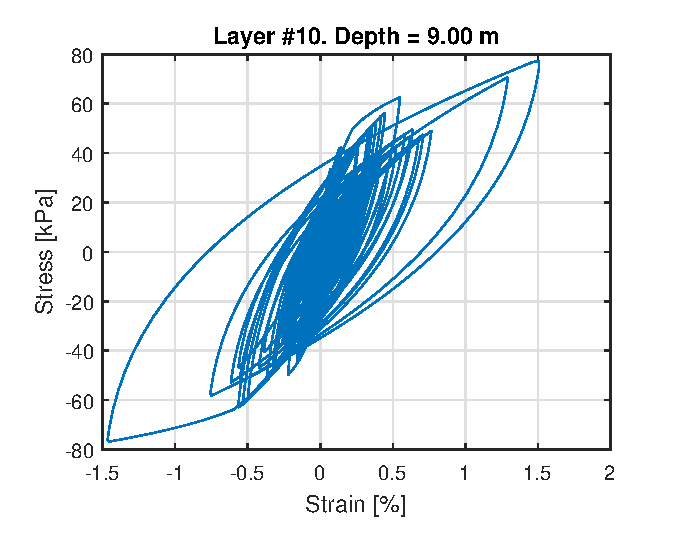
\includegraphics[width=0.49\textwidth]{stress_strain_loops.eps}}
	\subfloat{
	\includegraphics[width=0.49\textwidth]{view_movie.png}}
\end{figure}

\newpage
\section{Technical Manual}\label{sec:manual}

\subsection{Linear method}\label{sec:linear}

In linear approach, the soil is assumed as a Kelvin-Voigt solid, whose dynamic behavior is is described using a purely elastic spring and a purely viscous dashpot\footnote{Kramer, S. L. (1996), \emph{Geotechnical Earthquake Engineering}, Prentice Hall, Upper Saddle River, New Jersey.}, having two defining parameters, $G$ (soil modulus) and $\xi$ (soil damping ratio). Linear approach assumes $G$ and $\xi$ to remain unchanged in dynamic processes, which is not the case, especially when the ground motion intensity is strong.

\subsubsection{Frequency domain linear method}

In frequency domain linear analysis, the amplification of ground motions by the soil layers are computed via transfer functions, using the following formula,
\begin{equation}\label{eq:freq-domain-amplification}
    a_{\text{out}}\left(t\right)=\text{IFT}\left[H\left(\omega\right)\cdot\text{FT}\left[a_{\text{in}}(t)\right]\right]
\end{equation}
where $a_{\text{in}}(t)$ and $a_{\text{out}}$ are the input and output ground motions in time domain, FT[ ] and IFT[ ] represent Fourier transform and inverse Fourier transform, and $H(\omega)$ is the complex-valued transfer function in frequency domain, which can be solely determined by the soil property profile.

The following paragraphs show the derivation of $H(\omega)$ from the soil properties.

Let $ j $ denote the soil layer index, and $ A_j $ and $ B_j $ the upgoing and downgoing SH wave displacement amplitudes at the $ j $-th layer.  In this case, the following relationship holds for every $ j $:
\begin{equation}
 \left\{\begin{array}{c}
A_{j+1} \\
B_{j+1}
\end{array} \right\} = \left[\begin{array}{cc}
\f{1}{2}(1+\alpha^*_j)\mrm{e}^{ik^*_jh_j} & \f{1}{2}(1-\alpha^*_j)\mrm{e}^{-ik^*_jh_j} \\
\f{1}{2}(1-\alpha^*_j)\mrm{e}^{ik^*_jh_j} & \f{1}{2}(1+\alpha^*_j)\mrm{e}^{-ik^*_jh_j}
\end{array} \right]\cdot \left\{\begin{array}{c}
A_j \\
B_j
\end{array} \right\}  \eqdef \mathbf{D}_j\cdot \left\{\begin{array}{c}
A_j \\
B_j
\end{array} \right\}
\end{equation}
where $ \alpha_j^* = \displaystyle\f{\rho_j V^*_{s,j}}{\rho_{j+1} V^*_{s,j+1}}$ is the complex impedance ratio of two successive layers $ j $ and $ (j+1) $;  \newline $ V^*_{s,j} = V_{s,j}\cdot\sqrt{1+2i\xi_j}$ is the complex shear wave velocity of layer $ j $; $ h_j $ is the thickness of layer $ j $; and $ k^*_j = \displaystyle\f{\omega}{V^*_{s,j}} = \f{k_j}{1+i\xi_j}$ is the complex wave number of layer $ j $, where $ \omega $ is the angular frequency.

Hence
\begin{equation}
	\left\{\begin{array}{c}
A_j \\
B_j
\end{array} \right\} = \mathbf{D}_{j-1} \left\{\begin{array}{c}
A_{j-1} \\
B_{j-1}
\end{array} \right\} = \mathbf{D}_{j-1}\mathbf{D}_{m-2}\left\{\begin{array}{c}
A_{j-2} \\
B_{j-2}
\end{array} \right\} = \cdots = \mathbf{D}_{j-1}\mathbf{D}_{j-2}\cdots\mathbf{D}_{1}\left\{\begin{array}{c}
A_{1} \\
B_{1}
\end{array} \right\}
\label{eq:j_to_1}
\end{equation}
where $ A_1 = B_1 = S/2 $, and $ S $ is the total surface displacement amplitude.

Let $ \mathbf{E}_{j-1} = \mathbf{D}_{j-1}\mathbf{D}_{j-2}\cdots\mathbf{D}_{1} $, thus Equation~\eqref{eq:j_to_1} becomes
\begin{equation}\label{eq:j-to-1b}
\left\{\begin{array}{c}
A_j \\
B_j
\end{array} \right\} = \mathbf{E}_{j-1}\left\{\begin{array}{c}
A_1 \\
B_1
\end{array} \right\}  = \left[\begin{array}{cc}
E_{j-1}^{\langle 11\rangle} & E_{j-1}^{\langle 12\rangle} \\
E_{j-1}^{\langle 21\rangle} & E_{j-1}^{\langle 22\rangle}
\end{array} \right]\left\{\begin{array}{c}
S/2\\
S/2
\end{array} \right\}
\end{equation}

Equation~\eqref{eq:j-to-1b} relates the displacement amplitudes at the top of the $j$-th layer to the layer on ground surface. Using this equation we can also relate the displacement amplitudes of any two layers, $j$ and $k$,
\begin{equation}
    \left\{\begin{array}{c}
    A_j \\
    B_j
    \end{array} \right\} = \mathbf{E}_{j-1}\cdot\mathbf{E}_{k-1}^{-1}\cdot\left\{\begin{array}{c}
    A_k \\
    B_k
    \end{array} \right\}
\end{equation}
And if $m$ is the total number of soil layers (excluding the underlying bedrock), the displacement amplitudes between the top of bedrock and the top of ground surface is
\begin{equation}\label{eq:m-to-1}
\left\{\begin{array}{c}
A_m \\
B_m
\end{array} \right\} = \mathbf{E}_{m-1}\left\{\begin{array}{c}
A_1 \\
B_1
\end{array} \right\}  = \left[\begin{array}{cc}
E_{m-1}^{\langle 11\rangle} & E_{m-1}^{\langle 12\rangle} \\
E_{m-1}^{\langle 21\rangle} & E_{m-1}^{\langle 22\rangle}
\end{array} \right]\left\{\begin{array}{c}
S/2\\
S/2
\end{array} \right\}
\end{equation}

Referring to Figure~\ref{fig:three-types-of-input-motions}, three types of transfer functions can be written,


\begin{figure}[h]
    \centering
  \includegraphics[width=0.45\textwidth]{three_motion_types.png}\\
  \caption{Three types of input motions}\label{fig:three-types-of-input-motions}
\end{figure}

\textsf{(A)} The ``surface to borehole'' (surface motion to total borehole motion) transfer function:
\begin{equation}
H_{\text{A}}(\omega)  = \displaystyle\frac{\text{Ampl}(u_1)}{\text{Ampl}(u_{m-\text{(total)}})} = \frac{S/2 + S/2}{A_m+B_m} = \frac{2}{E_{m-1}^{\la 11\ra} + E_{m-1}^{\la 12\ra}+E_{m-1}^{\la 21\ra} + E_{m-1}^{\la 22\ra}}
\end{equation}
%and the absolute value of $H_{\text{A}}(\omega)$ is the amplification factor
%\begin{equation}
%\mathrm{AF}_{\txt{S-BH}}(\omega) = |\mathrm{TF}_{\txt{S-BH}}(\omega)| = \f{2}{\left|E_{N-1}^{\la 11\ra} + E_{N-1}^{\la 12\ra}+E_{N-1}^{\la 21\ra} + E_{N-1}^{\la 22\ra}\right|}
%\end{equation}

\textsf{(B)} The ``surface to incident'' (surface motion to incident motion at borehole) transfer function is
\begin{equation}
H_{\text{B}}(\omega) = \f{S/2+S/2}{A_m} =\f{2}{E_{m-1}^{\la 11\ra} + E_{m-1}^{\la 12\ra}}
\end{equation}

\textsf{(C)} The ``surface to rock outcrop'' (motion at soil surface to motion at rock outcrop site's surface) transfer function is
\begin{equation}
H_{\text{C}}(\omega) = \f{S/2+S/2}{2A_m} = \f{1}{E_{m-1}^{\la 11\ra} + E_{m-1}^{\la 12\ra}}
\end{equation}

The three types of amplification functions of a same site, plotted together on the same graph, are shown in Figure~\ref{fig:three-types-of-TF}.

\begin{figure}[h]
    \centering
  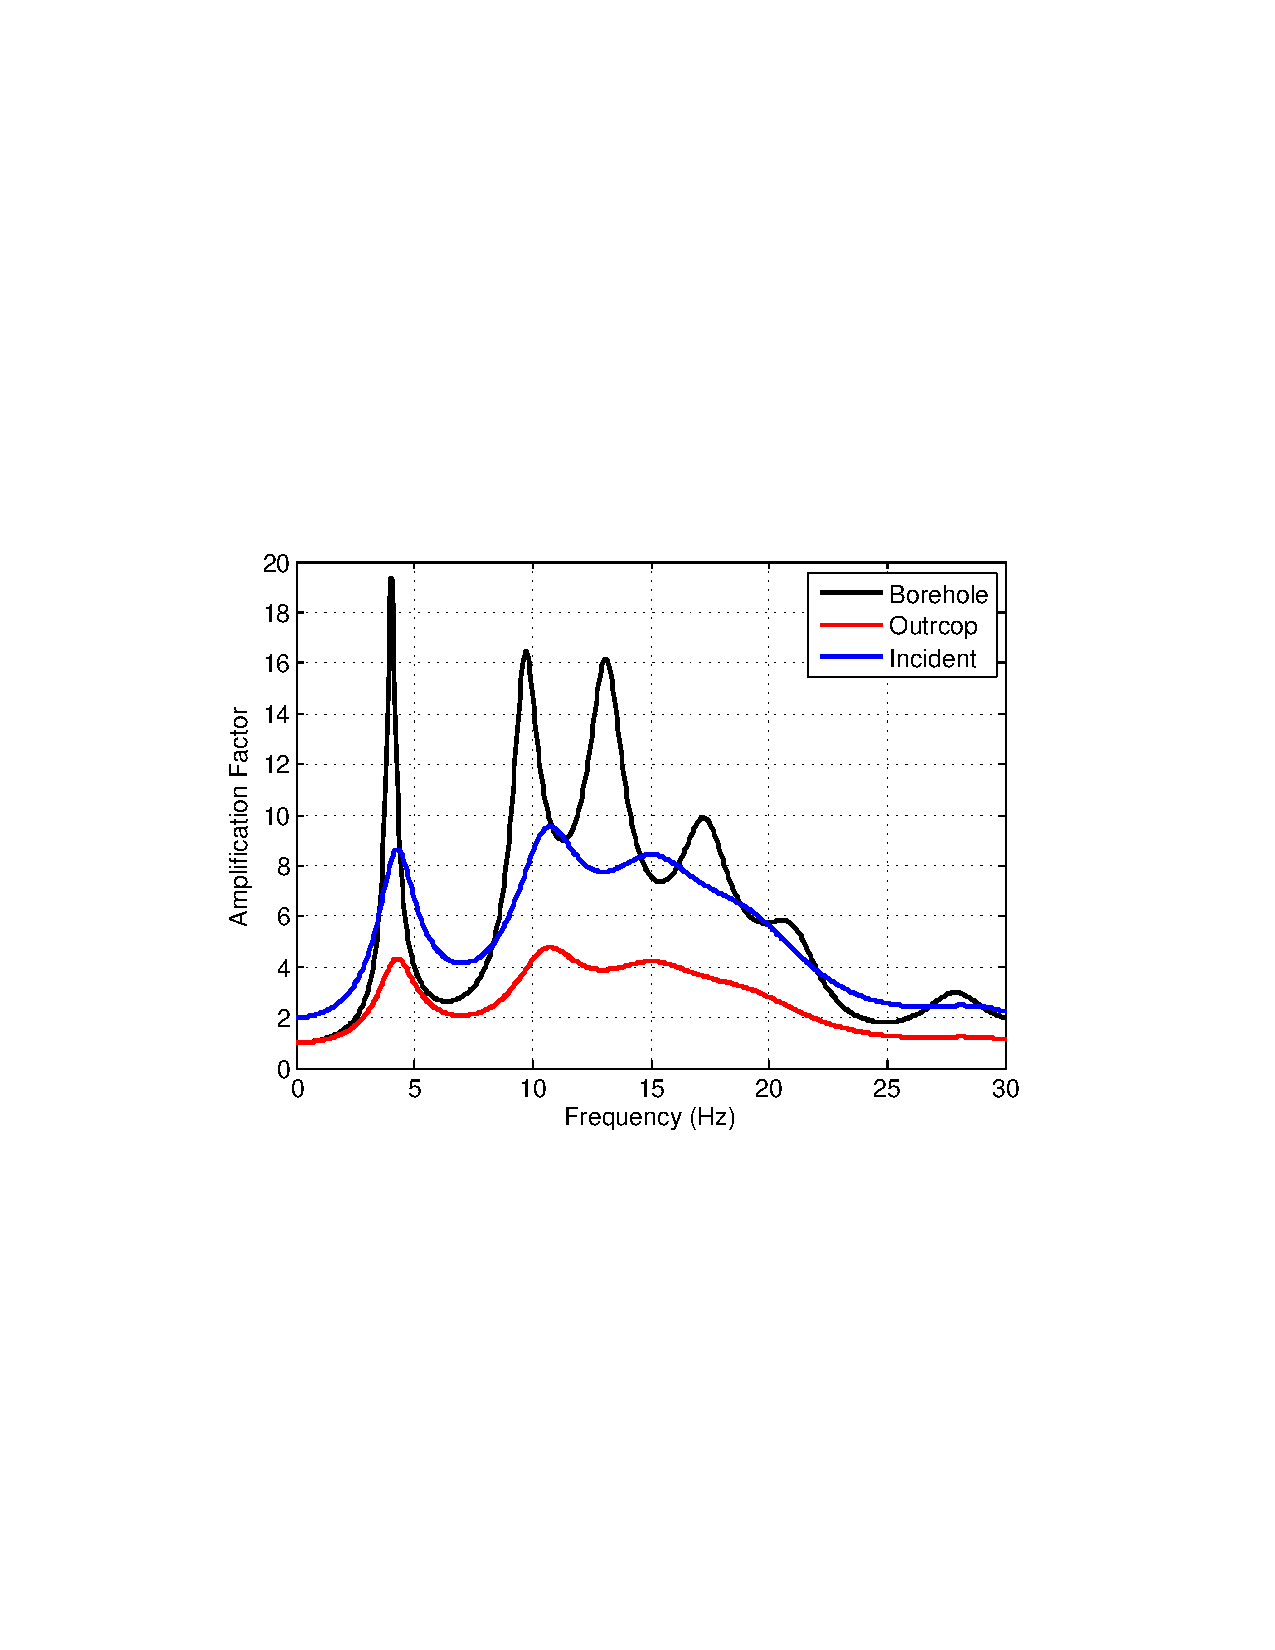
\includegraphics[width=0.6\textwidth]{three_types_of_TF.pdf}\\
  \caption{Three types of linear transfer functions}\label{fig:three-types-of-TF}
\end{figure}




\subsubsection{Time domain linear method}

The time domain linear approach solves the wave propagation functions directly in the time domain, using the finite difference scheme. The soil properties remain unchanged during the entire duration of shaking. In order to incorporate $G$ and $\xi$ information from the input into the time domain scheme, a numerical model aiming at approximating the frequency independent damping behavior of soil is used. The degree of approximation is satisfactory, however not perfect. Therefore there is a slight difference between the result of frequency domain linear approach and time domain linear approach.

The merit of time domain linear approach is that it prevents the ``wrap-around'' phenomenon that frequency-domain linear approach sometimes has. Because of the underlying assumption of Fourier transform, that the signal in time domain being transformed ``starts from the beginning of time and lasts forever'', the response that corresponds to the end of the input ground motion appears at the beginning part of the output ground motion, i.e., ``wrapped-around''.  This phenomenon is especially pronounced when the input ground motion is synthetic and short, e.g., a Ricker wavelet.

For more details concerning how the temporal-spatial finite difference is carried out, please refer to Section~\ref{sec:nonlinear} on page \pageref{sec:nonlinear}.


\subsection{Equivalent linear method}\label{sec:equivalent-linear}

\subsubsection{Original equivalent linear method}

The equivalent linear approach, originally proposed by Harry Bolton Seed and Izzat M.~Idriss in 1970, and first programmed in SHAKE (Schnabel et al., 1972; Idriss \& Sun, 1992), is a modified linear approach which partly incorporates the nonlinear properties of soil. This approach accepts that modulus and damping of soil in a dynamic process are no longer the same as their initial values, which are $G_{\text{max}}$ and $\xi_{\text{small strain}}$. In order to determine the appropriate values for $G$ and $\xi$, the equivalent linear approach calculates linear site response (in frequency domain) once, obtaining the strain time histories at the center of each soil layer. Then, an ``effective'' strain value is picked for each layer, which is subsequently used to obtain an updated $G$ value and an updated $\xi$ value from the modulus reduction and damping curves. Linear site response is carried out once more, obtaining updated strain time histories and effective strains, which are used to update $G$ and $\xi$ again.  This process is repeated until convergence. The ground response after convergence is the result of the equivalent linear approach.

The detailed procedure of the equivalent linear approach in SeismoSoil is as follows.
\begin{enumerate}
    \item Re-discretize the existing soil layers based on shear wave velocities of each layer (for details, see Section~\ref{sec:rediscretization} on page \pageref{sec:rediscretization})
    \item Calculate linear transfer functions between each intermediate layer and the input point (can either be ``borehole'', or ``incident'', or ``outcrop'')
    \item Use Equation~\eqref{eq:freq-domain-amplification} to calculate acceleration time histories on the top of each soil layer
    \item Integrate acceleration time histories twice to get displacement time histories
    \item Use the displacements between two neighboring layers to calculate the approximate strain time histories at the mid-point of each layer
    \item Pick 65\% of the maximum absolute strain as the ``effective'' strain (for every layer)
    \item Pick updated $G$ and $\xi$ values according to the ``effective'' strains of each layer
    \item Check if the relative differences between two successive $G$ and $\xi$ values fall below 7.5\% (for every layer)
    \item If true, end the iteration; of not, repeat steps 2--8
    \item After 10 iterations, break out of the loop, regardless of convergence
\end{enumerate}

The equivalent linear approach does not reflect the real-world soil behavior in that it assumes constant $G$ and $\xi$ values for each layer, during the entire duration of the dynamic response. In fact, modulus and damping of soil change instantaneously with the strain level that the soil has. Also, different frequency components in the input motion are associated with different strain levels, thus increasing damping values indiscriminatively causes the high frequency components in a ground motions, which are usually not as intense as the low frequency ones, to attenuate excessively. This is especially obvious for deep and soft sites.

An example of linear, equivalent linear and true amplification factors is shown in Figure~\ref{fig:af_comparison}. The true amplifications factor is calculated from actual surface and borehole seismographs. From the figure, we can see that how much equivalent linear approach overdamps the high frequency components, and how linear approach might overestimate ground response at some particular frequencies.

\begin{figure}[h]
    \centering
  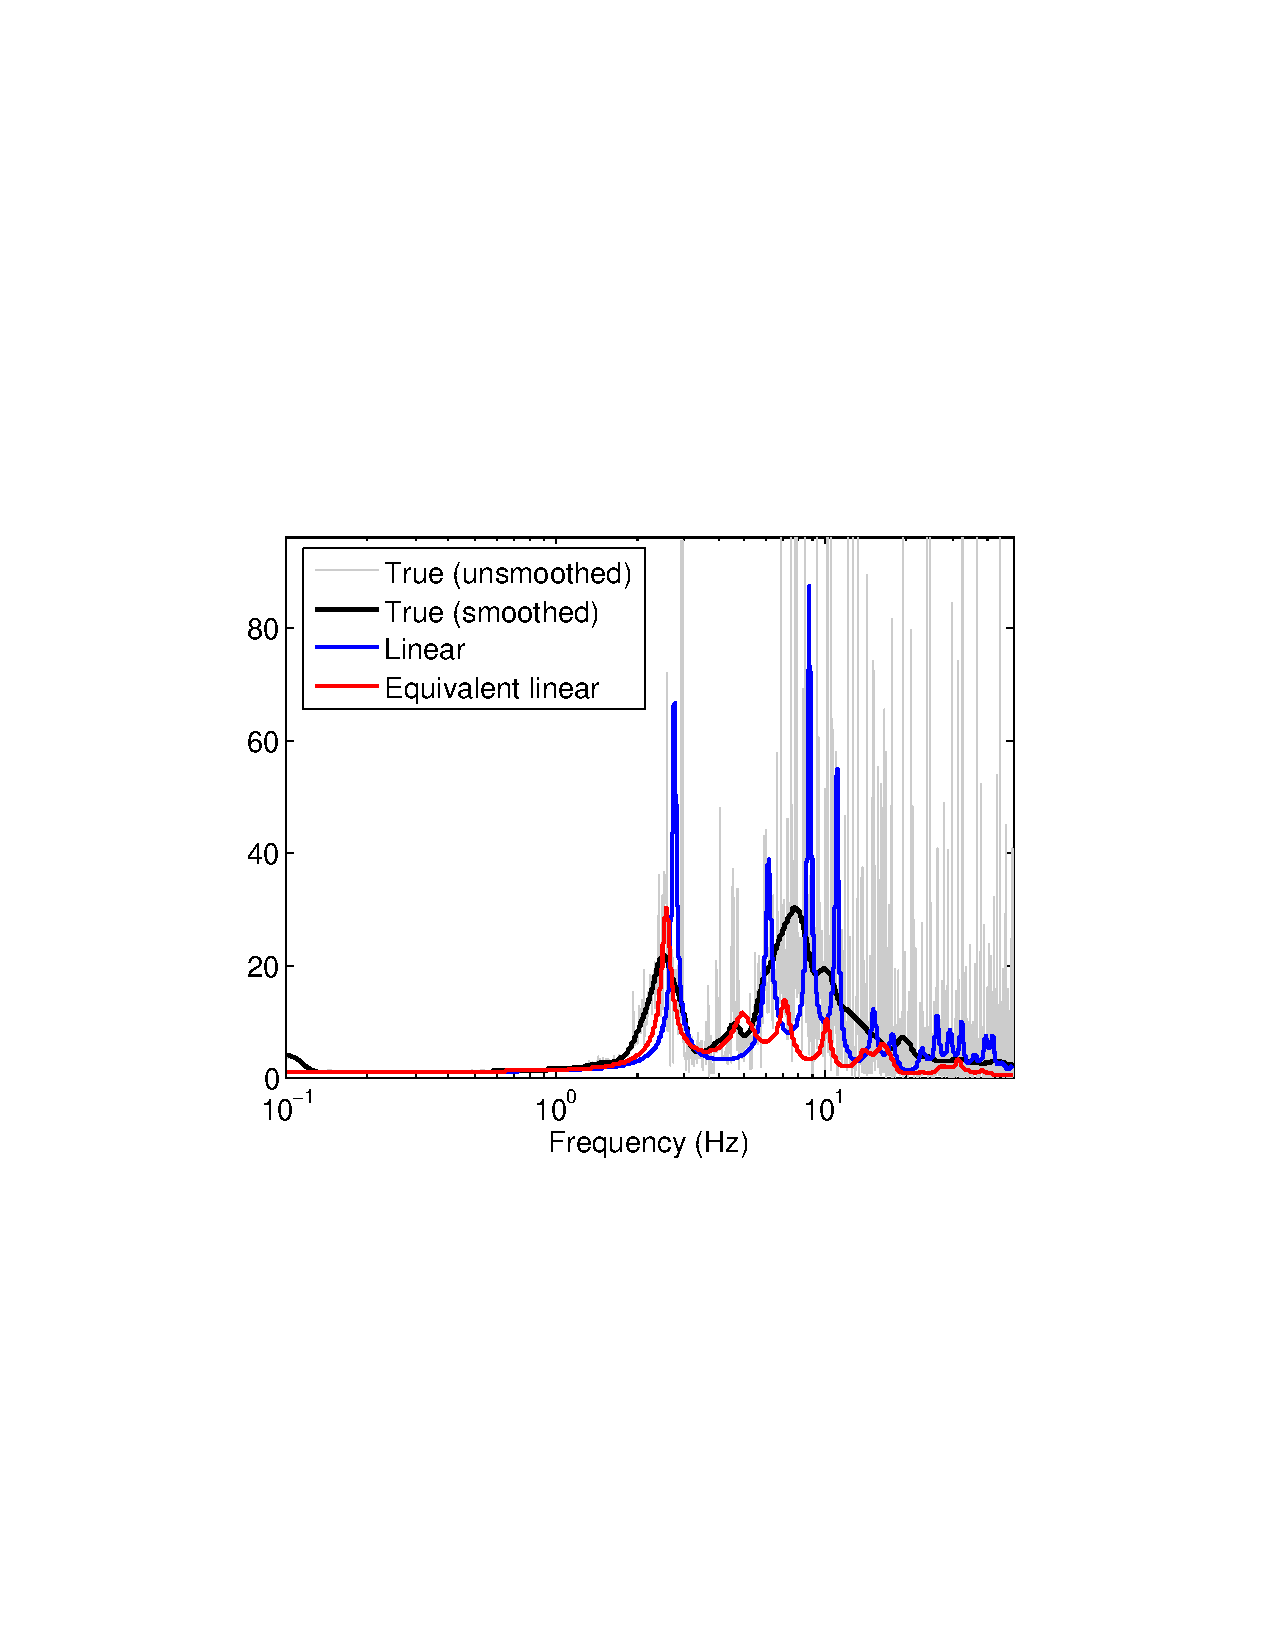
\includegraphics[width=0.5\textwidth]{amplification_factor_comparison.pdf}\\
  \caption{Comparison of amplifications factors. The ``true'' amplification factor is calculated from actual recordings.}\label{fig:af_comparison}
\end{figure}




%Modulus and damping curves of soils are used to determine new parameters for each soil layer. The frequency domain linear approach, same as previously discussed in Section~\ref{sec:linear}, is repeated to get an updated displacement time history and strain time history



%, and iterations are performed until convergence. This stepwise analysis procedure has been formalized into a computer code termed SHAKE \citep{Schnabel1972SHAKE}, which currently is the most widely used analysis package for 1D site-specific response calculations. The advantages of the equivalent-linear approach are that the mathematical simplicity of linear analysis is preserved and the determination of nonlinear parameters is avoided.

%Despite the effectiveness of the approach for the analysis of relatively stiff sites subjected to inter-mediate levels of strain (<$10^{-3}$), however, the equivalent linear method has been shown to overestimate the peak ground acceleration for large events, and artificially suppress the high frequency components when applied for the analysis of deep sites. An alternative methodology that accounts for the frequency-dependence of strain amplitudes and associated dynamic soil properties has been proposed by \citet{Assimaki_Kausel_2002}, and has been shown to yield more satisfactory results for deep sedimentary deposits; the applicability of the alternative formulation, however, is still limited to the medium strain levels \citep{Hartzell2004BSSA}.
%The linear stress-strain material behavior and total stress approach associated with equivalent linear models, entirely prohibits their use for problems that involve large levels of strain (e.g. near-fault motions), deep and/or soft and very soft sedimentary sites. We here implement only the original formulation of the equivalent linear method for ground surface response analyses at each station to the ensemble of ground motion time-histories. Comparison of the equivalent linear analyses results to the fully nonlinear response described below reveals the drawbacks of equivalent linear analyses associated with overdamping of high frequency components, and highlights the sites and ground motion characteristics that dictate the use of nonlinear models for the computation of site-specific amplification factors.


\subsubsection{Equivalent linear method with frequency dependent modulus and damping}

The most obvious disadvantage of the original equivalent linear method is that it artificially suppresses higher frequencies, i.e., the higher frequency components in the simulated ground motion is unrealistically low compared to true outputs. Assimaki and Kausel (2002) proposed a frequency- and pressure-dependent equivalent linear method, which significantly improved the predictions of higher frequency contents. For the technical details of this method, please refer to the original paper:

Assimaki and Kausel (2002) ``An equivalent linear algorithm with frequency- and pressure-dependent moduli and damping for the seismic analysis of deep sites''. \emph{Soil Dynamics and Earthquake Engineering}. Vol.~22, 959--965. (http://www.sciencedirect.com/science/article/pii/S0267726102001203)

The kernel of this method within SeismoSoil is written in Fortran by Fabian Bonilla, for which the authors are very grateful.

\subsection{Nonlinear method}\label{sec:nonlinear}

The nonlinear analysis is performed in the time domain, using finite difference method (FDM). The features of our nonlinear method are
\begin{itemize}
	\item A memory-variable technique proposed by Liu and Archuleta (2006)\footnote{Liu, P.-C., and R.~J.~Archuleta (2006), Efficient modeling of Q for 3D numerical simulation of wave propagation, \emph{Bulletin of the Seismological Society of America}, 96(4A), 1352--1358.} to model small-strain damping is used, which, compared to Rayleigh and Caughey damping (both are frequency dependent), better simulates the frequency-independent small-stain damping in reality;
	
	\item The hysteresis (i.e., unloading/reloading) behavior model, proposed by Li and Assimaki (2010)\footnote{Li, W., and D.~Assimaki (2010), Site- and motion-dependent parametric uncertainty of site-response analyses in earthquake simulations, \emph{Bulletin of the Seismological Society of America}, 100(3), 954--968.}, based on the original model by Muravskii (2005)\footnote{Muravskii, G. (2005), On description of hysteretic behavior of materials, \emph{International Journal of Solids and Structures}, 42, 2625--2644.}, is capable of simultaneously matching $G/G_{\max}$ and damping curves, yielding narrower and more realistic hysteresis loops than the loops by Masing rules.
	
	\item The stress-strain and damping behaviors of the soils are described by the modified hyperbolic (MKZ) model (Matasovic and Vucetic, 1993\footnote{Matasovic, J., and M.~Vucetic (1993), Cyclic characterization of liquefiable sands, \emph{Journal of Geotechnical Engineering}, 119(11), 1805--1822.}).
\end{itemize}

The illustration below (modified from Bardet, 2001) shows the spatial discretization of the FDM scheme.

\begin{figure}[H]
	\centering
	\includegraphics[width=0.99\textwidth]{FDM_scheme.png}\\
	%\caption{Comparison of amplifications factors. The ``true'' amplification factor is calculated from actual recordings.}\label{fig:af_comparison}
\end{figure}

\newpage
\subsection{Miscellaneous technical details}

\subsubsection{Baseline correction}\label{sec:baseline-correction}

For various reasons, there are usually baseline offsets in the acceleration recordings, resulting in non-realistic shifts in the velocity and displacement time histories integrated from acceleration. To address this issue, we use high-pass filtering to remove the low frequency components in the acceleration recordings.

The procedures are as follows:
\begin{itemize}
	\item Remove ``pre-event'' mean value, which is defined as the average acceleration of the ``silent'' part 
	           of the recording, where the acceleration should be zero
	\item Cut off the beginning and end of the motion using the first zero-crossings as bounds
	\item Pad zeros at both ends of the acceleration array
	\item Apply zero-phase high-pass filtering (default cut-off frequency: 0.2~Hz; users can use other values)
	\item Adjust the filtered time series so that it is aligned chronologically with the original time series
\end{itemize}

The result of the baseline correction is shown in Figure~\ref{fig:baseline_result_duplicate}.% The advantage of the baseline correction in SeismoSoil is that the corrected signal is in sync with the uncorrected signal, and has the same number of data points.

\begin{figure}[H]
	\centering
	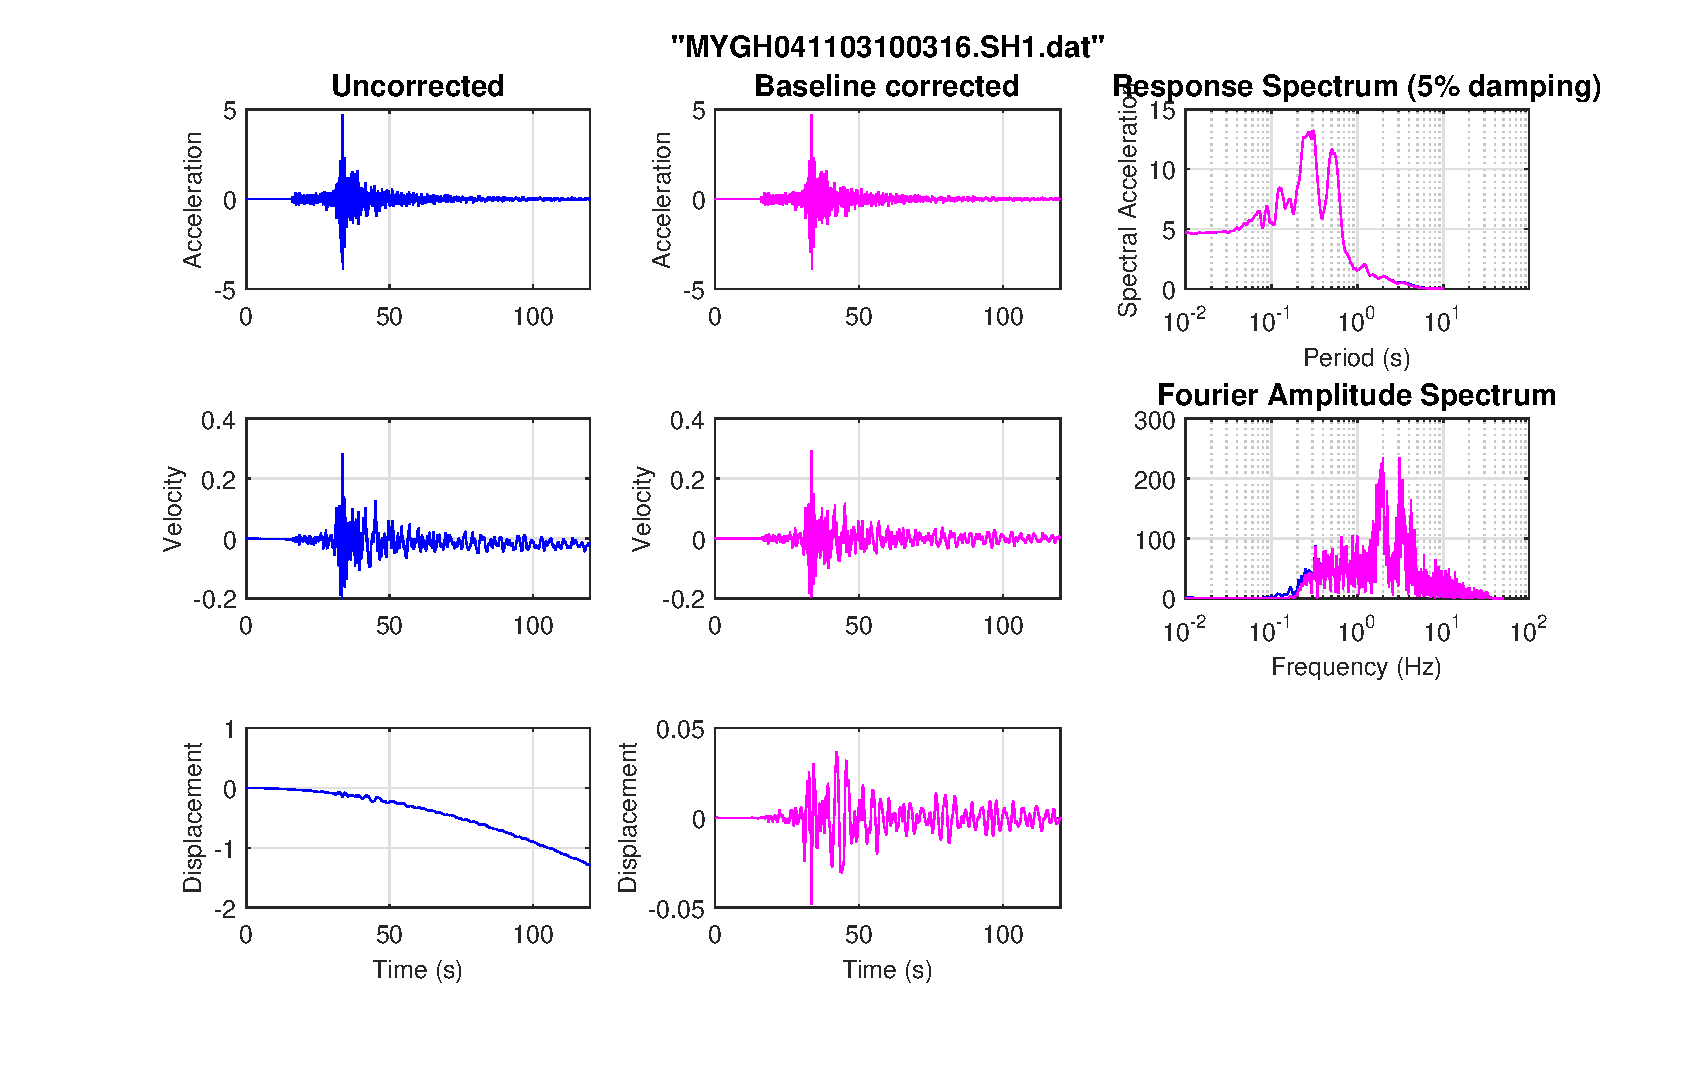
\includegraphics[width=.99\textwidth]{baseline_correction_result_new.eps}\\
	\caption{Baseline correction result}
	\label{fig:baseline_result_duplicate}
\end{figure}

\subsubsection{Konno-Ohmachi smoothing of frequency spectra}\label{sec:konno-ohmachi}

Spectral ratios calculated from surface-borehole ground motion pairs of actual recordings, or from output-input accelerations of the time-domain nonlinear analysis, usually have lots of spikes due to ``discrete spectral holes'' in the Fourier spectrum at the denominator. A smoothing window applied to the spectral ratio is able to address this problem, making the spectral ratio more intuitive and understandable.

\begin{figure}[h]
	\centering
	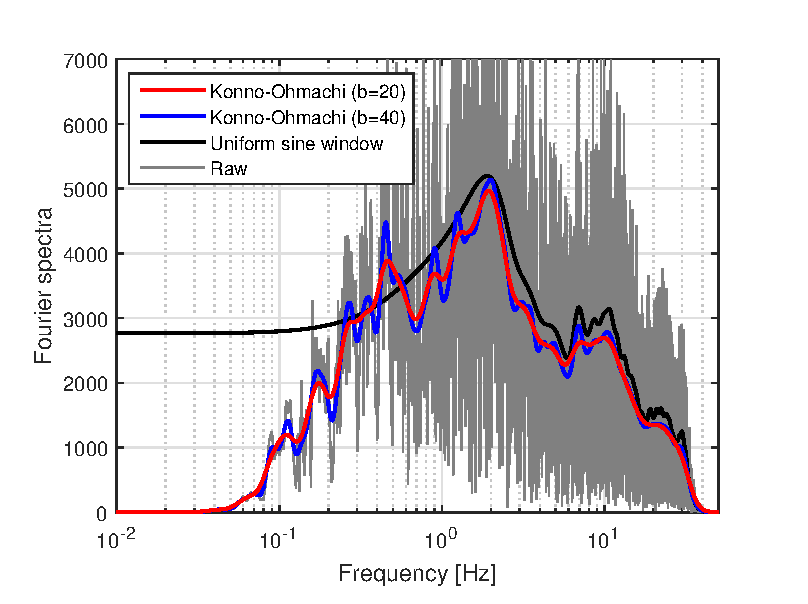
\includegraphics[width=0.65\textwidth]{different_smoothing_windows.eps}
	\caption{Comparison of different smoothing windows}\label{fig:different_smoothing_windows}
\end{figure}

Some traditionally used of smoothing windows include uniform window, triangle window, or sine window (as the black line in Figure~\ref{fig:different_smoothing_windows}), which has the same span to the left and the right of the point to be smoothed. This type of window has the same ``smoothing intensity'' for all frequencies, which will be later referred to as the ``linear-span smoothing''

 However, since the spectral ratios are often plotted in log-frequency scales, and the spikes are usually more pronounced at higher frequencies (above 5--10~Hz), it is advantageous to use a class of smoothing windows that has the same left and right span in logarithmic scale. The Konno-Ohmachi smoothing window\footnote{Konno, K.~and T.~Ohmachi.~(1998) ``Ground-Motion Characteristics Estimated from Spectral Ratio between Horizontal and Vertical Components of Microtremor''. \emph{Bulletin of the Seismological Society of America}, Vol.~88, No.~1, pp.~228--241.} is one of this kind. The function for Konno-Ohmachi smoothing window is
\begin{equation}\label{eq:konno-ohmachi}
	w(f,f_c) = \left(   \frac{ \sin\left(  b\log_{10}(f/f_c)  \right) }{ b\log_{10}(f/f_c) }   \right)^4
\end{equation}
where $f_c$ is the frequency at which the spectral ratio will be smoothed, $f$ is the frequency variable, and $b$ is the smoothing factor which adjusts the width of $w(f,f_c)$. The larger $b$ is, the less ``intense'' the smoothing would be. In SeismoSoil, the default $b$ value is $40$.





Figure~\ref{fig:different_smoothing_windows} shows a comparison of a raw (unsmoothed) spectral ratio, a linear-span smoothed (uniform sine window), and two Konno-Ohmachi smoothed ($b=20$ and $40$). From the figure, we can see that the linear-span smoothing does not smooth the high-frequency (above 5~Hz) components enough, thus the two fundamental frequency modes cannot be clearly observed. On the other hand, Konno-Ohmachi smoothing does a better job in eliminating the spectral spikes at higher frequencies, which are mainly numerical artifacts.



However, the users should note that the choice of smoothing functions should serve the purpose of the smoothing, Konno-Ohmachi smoothing is appropriate for spectral ratios, but might produce physically meaningless results for other applications.




\subsubsection{Automatic re-discretization of soil layers}\label{sec:rediscretization}

The time-domain methods in SeismoSoil are finite difference methods (FDM), and hence the spatial discretization size directly relates to the accuracy of the numerical scheme. Referring to Figure~\ref{fig:spatial_discretization}, at least 5 points are needed to crudely ``represent'' trend of a full sine wave, and 10 points can reconstruct the sine wave to a satisfactory degree. Therefore, the spatial grid size in SeismoSoil is
\[
\Delta h = \lambda/10
\]
where $ \lambda $ is the wavelength of the sine wave.

\begin{figure}[h]
	\centering
	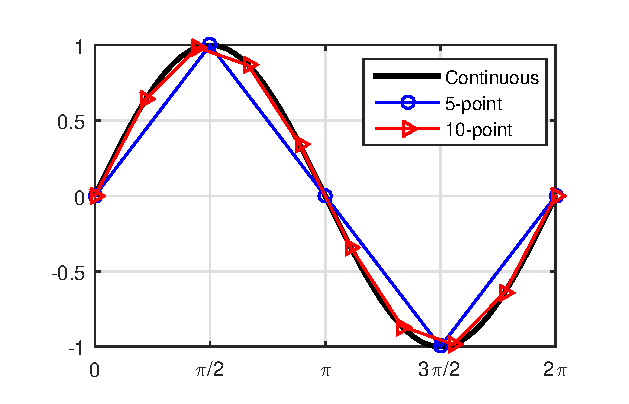
\includegraphics[width=0.55\textwidth]{spatial_discretization.eps}\\
	\caption{Example of different spatial discretization}\label{fig:spatial_discretization}
\end{figure}

The value of $ \lambda $ is different for different frequencies:
\[
\lambda = V_S/f
\]
where $ f $ is the frequency of the harmonic wave component, and $ V_S $ is the shear wave velocity of a specific layer. The default maximum frequency that SeismoSoil is set to resolve is 30~Hz, thus
\[
\Delta h \,\,[\mathrm{m}] = \frac{V_S\,\,[\mathrm{m/s}]}{300\,\mathrm{sec}^{-1}}
\]


Layers with smaller $ V_S $ will be discretized to finer sublayers. This process is done internally within SeismoSoil.

If the users have needs for simulating frequencies higher than 30~Hz, please contact the authors.




\subsubsection{Deconvolution of rock-outcrop motions}\label{sec:deconvolution}

Oftentimes, the rock-outcrop motions, or the ``reference station'' motions, are used as the input motion to calculate the response of the softer soil site (see Figure~\ref{fig:three-types-of-input-motions} on page~\pageref{fig:three-types-of-input-motions}). The rock has a low value of damping ratio, therefore using rock-outcrop motions as input motions is acceptable, but not exactly accurate. If the rock properties (i.e., $V_S$, damping ratio) are known, and also the depth of the soil deposit is known, the users are advised to deconvolve (i.e., ``propagate downwards'') the rock-outcrop motion to the rock-soil interface, and then use the motion as the input incident motion. This results in a slightly stronger input motion, because the energy loss within the rock is accounted for and corrected.



\section{List of references}


Assimaki and Kausel (2002) ``An equivalent linear algorithm with frequency- and pressure-dependent moduli and damping for the seismic analysis of deep sites''. \emph{Soil Dynamics and Earthquake Engineering}. Vol.~22, 959--965.

Darendeli, M.~B.~(2001). ``Development of a new family of normalized modulus reduction and material damping curves.'' Pages 220--272, \emph{PhD thesis}, The University of Texas at Austin.

Konno, K.~and T.~Ohmachi.~(1998) ``Ground-Motion Characteristics Estimated from Spectral Ratio between Horizontal and Vertical Components of Microtremor''. \emph{Bulletin of the Seismological Society of America}, Vol.~88, No.~1, pp.~228--241.

Kramer, S. L. (1996), \emph{Geotechnical Earthquake Engineering}, Prentice Hall.

Li, W., and D.~Assimaki (2010), Site- and motion-dependent parametric uncertainty of site-response analyses in earthquake simulations, \emph{Bulletin of the Seismological Society of America}, 100(3), 954--968.

Liu, P.-C., and R.~J.~Archuleta (2006), Efficient modeling of Q for 3D numerical simulation of wave propagation, \emph{Bulletin of the Seismological Society of America}, 96(4A), 1352--1358.

Matasovic, J., and M.~Vucetic (1993), Cyclic characterization of liquefiable sands, \emph{Journal of Geotechnical Engineering}, 119(11), 1805--1822.

Muravskii, G. (2005), On description of hysteretic behavior of materials, \emph{International Journal of Solids and Structures}, 42, 2625--2644.

Seed, H. B., and I. M. Idriss (1970b), Soil moduli and damping factors for dynamic response analyses, \emph{UCB/EERC- 70/10}, Earthquake Engineering Research Center, University of California at Berkeley.


\end{document} 